\documentclass[10pt]{article}
\usepackage[polish]{babel}
\usepackage[utf8]{inputenc}
\usepackage[T1]{fontenc}
\usepackage{amsmath}
\usepackage{amsfonts}
\usepackage{amssymb}
\usepackage[version=4]{mhchem}
\usepackage{stmaryrd}
\usepackage{graphicx}
\usepackage[export]{adjustbox}
\graphicspath{ {./images/} }

\title{III Konkurs Matematyczny St@ś \\
 XIV LO im. Stanisława Staszica \\
 29 kwietnia 2003 roku }

\author{}
\date{}


\begin{document}
\maketitle
\section*{klasa V}
Na rozwiazanie poniższych zadań masz 90 minut. Kolejność rozwiqzywania tych zadań jest dowolna. Wszystkie zadania sa jednakowo punktowane. Maksymalnq liczb̨ punktów może uzyskać jedynie peine mzaiqzanie, z uzasadnieniem i odpowiedziq.\\
Używanie korektora i korzystanie z kalkulatora jest niedozwolone.

\section*{Zadanie 1.}
Na stole leżą 2003 monety. Jaś w jednym ruchu może wziąć dokładnie 3, 36 lub 69 monet. Czy Jaś, wykonując wiele takich ruchów, może wziąć wszystkie monety ze stolu?

\section*{Zadanie 2.}
Która liczba jest większa: \(\frac{12345677}{12345678}\) czy \(\frac{123456788}{123456789}\) ?

\section*{Zadanie 3.}
Dwa boki trójkąta mają długości 3,14 i 0,67 . Długość trzeciego boku tego trójkąta jest liczbą naturalną. Oblicz długość tego trzeciego boku.

\section*{Zadanie 4.}
Wszystkie wierzchołki pewnego sześciokąta foremnego leżą na okręgu o promieniu 2 cm .\\
Oblicz obwód tego sześciokąta.

\section*{Zadanie 5.}
Sześcian rozcięto wzdłuż tych krawędzi, które na rysunku zaznaczono grubszą linią. Narysuj powstałą siatkę.\\
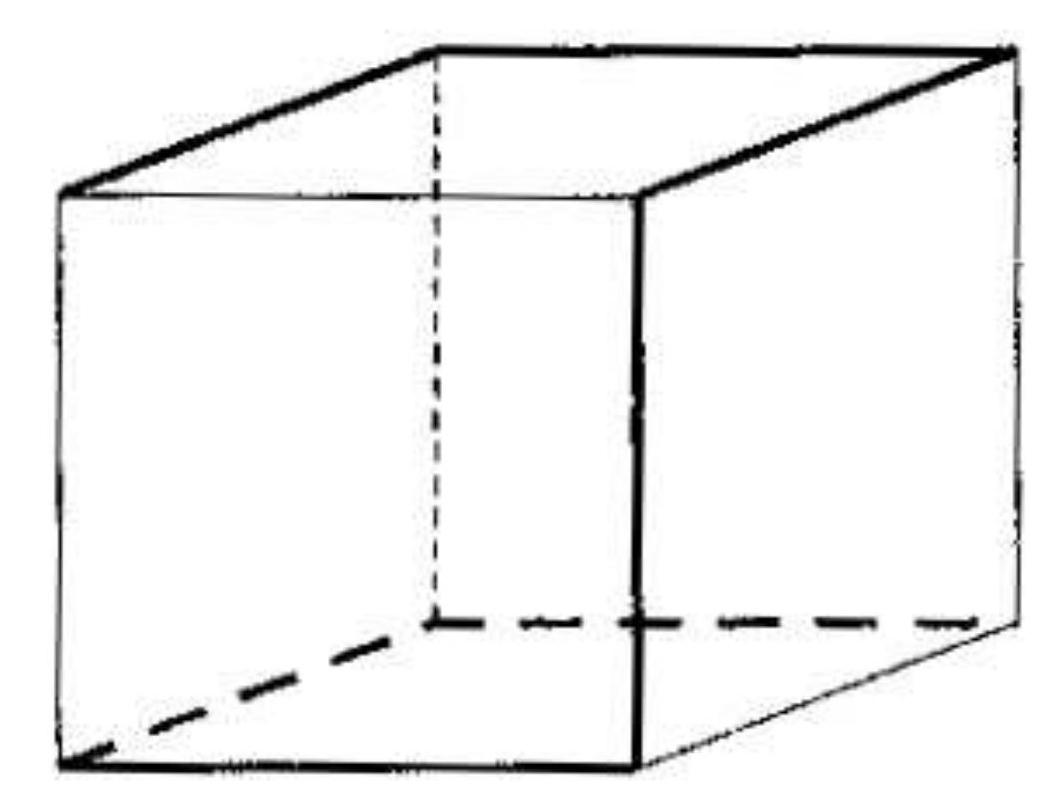
\includegraphics[max width=\textwidth, center]{2024_11_21_a8e98f1bc496eab22bc6g-1}


\end{document}